\documentclass[a4paper,11pt,fleqn,dvipsnames,twoside,openright]{memoir} 	% Openright aabner kapitler paa hoejresider (openany begge)

%%%% PACKAGES %%%%

% ¤¤ Oversaettelse og tegnsaetning ¤¤ %
\usepackage[utf8]{inputenc}					% Input-indkodning af tegnsaet (UTF8)
\usepackage[danish]{babel}					% Dokumentets sprog
\usepackage[T1]{fontenc}					% Output-indkodning af tegnsaet (T1)
\usepackage{ragged2e,anyfontsize}			% Justering af elementer
\usepackage{fixltx2e}						% Retter forskellige fejl i LaTeX-kernen

																			
% ¤¤ Figurer og tabeller (floats) ¤¤ %
\usepackage{graphicx} 						% Haandtering af eksterne billeder (JPG, PNG, EPS, PDF)
%\usepackage{eso-pic}						% Tilfoej billedekommandoer paa hver side
%\usepackage{wrapfig}						% Indsaettelse af figurer omsvoebt af tekst. \begin{wrapfigure}{Placering}{Stoerrelse}
\usepackage[space]{grffile}					% Bør gøre det muligt at have mellemrum i filnavne.
\usepackage{multirow}                		% Fletning af raekker og kolonner (\multicolumn og \multirow)
\usepackage{multicol}         	        	% Muliggoer output i spalter
\usepackage{rotating}						% Rotation af tekst med \begin{sideways}...\end{sideways}
\usepackage{colortbl} 						% Farver i tabeller (fx \columncolor og \rowcolor)
\usepackage[usenames,dvipsnames]{xcolor}	% Definer farver med \definecolor. Se mere: http://en.wikibooks.org/wiki/LaTeX/Colors
%\usepackage{flafter}						% Soerger for at floats ikke optraeder i teksten foer deres reference
\let\newfloat\relax 						% Justering mellem float-pakken og memoir
\usepackage{float}							% Muliggoer eksakt placering af floats, f.eks. \begin{figure}[H]
\setlength{\heavyrulewidth}{0.15em}			% Sætter \toprule og \bottomrule til fast størrelse (0.08 er default)
%\setlength{\lightrulewidth}{0.05em}		% Sætter \midrule til fast størrelse (0.05 er default)
\usepackage{array}							% Bruges i forbindelse med \newcolumntype-command under egne commands
\usepackage{pdfpages}						% Bruges så der kan indsættes pdf, som sider (se forside for eksempel)
\usepackage{tablefootnote}


% ¤¤ Matematik mm. ¤¤
\usepackage{amsmath,amssymb,stmaryrd} 		% Avancerede matematik-udvidelser
\usepackage{mathtools}						% Andre matematik- og tegnudvidelser
\usepackage{textcomp}                 		% Symbol-udvidelser (f.eks. promille-tegn med \textperthousand )
\usepackage{rsphrase}						% Kemi-pakke til RS-saetninger, f.eks. \rsphrase{R1}
\usepackage[version=3]{mhchem} 				% Kemi-pakke til flot og let notation af formler, f.eks. \ce{Fe2O3}
\usepackage{siunitx}						% Flot og konsistent praesentation af tal og enheder med \si{enhed} og \SI{tal}{enhed}
\sisetup{locale=DE}							% Opsaetning af \SI (DE for komma som decimalseparator) 

% ¤¤ Referencer og kilder ¤¤ %
\usepackage[danish]{varioref}				% Muliggoer bl.a. krydshenvisninger med sidetal (\vref)
\usepackage{natbib}							% Udvidelse med naturvidenskabelige citationsmodeller
\usepackage{xr-hyper}							% Referencer til eksternt dokument med \externaldocument{<NAVN>}
\externaldocument[DokRap-]{../Dokumentationsrapport/Dokumentationsrapport}	% Muliggør eksterne referencer til produktrapporten
%\usepackage{glossaries}					% Terminologi- eller symbolliste (se mere i Daleifs Latex-bog)



% ¤¤ Misc. ¤¤ %
\usepackage{lipsum}							% Dummy text \lipsum[..]
\usepackage[shortlabels]{enumitem}			% Muliggoer enkelt konfiguration af lister
\usepackage{pdfpages}						% Goer det muligt at inkludere pdf-dokumenter med kommandoen \includepdf[pages={x-y}]{fil.pdf}	
\pdfoptionpdfminorversion=6					% Muliggoer inkludering af pdf dokumenter, af version 1.6 og hoejere
\pretolerance=2500 							% Justering af afstand mellem ord (hoejt tal, mindre orddeling og mere luft mellem ord)

% Kommentarer og rettelser med \fxnote. Med 'final' i stedet for 'draft' udloeser hver note en error i den faerdige rapport.
\usepackage[footnote,draft,danish,silent,nomargin]{fixme}		


%%%% CUSTOM SETTINGS %%%%

% ¤¤ Marginer ¤¤ %
\setlrmarginsandblock{3.5cm}{2.5cm}{*}		% \setlrmarginsandblock{Indbinding}{Kant}{Ratio}
\setulmarginsandblock{2.5cm}{3.0cm}{*}		% \setulmarginsandblock{Top}{Bund}{Ratio}
\checkandfixthelayout 						% Oversaetter vaerdier til brug for andre pakker

%	¤¤ Afsnitsformatering ¤¤ %
\setlength{\parindent}{0mm}           		% Stoerrelse af indryk
\setlength{\parskip}{3mm}          			% Afstand mellem afsnit ved brug af double Enter
\linespread{1,1}							% Linie afstand
\newcommand{\tab}{\hspace*{2em}}			% ved \tab{} indrykkes det i klammerne ind
\usepackage{titlesec}							%Muliiggøre ændring af sections i alle lag
\titleformat*{\section}{\LARGE\bfseries\color{NavyBlue}}		%section = størst
\titleformat*{\subsection}{\Large\bfseries\color{RoyalBlue}}		%sub og subsub har samme størrelse
\titleformat*{\subsubsection}{\Large\bfseries}
\titleformat*{\paragraph}{\large\bfseries}		%Benyttes umiddelbart ikke
\titleformat*{\subparagraph}{\large\bfseries}	%Benyttes umiddelbart ikke

% ¤¤ Litteraturlisten ¤¤ %
\bibpunct[,]{[}{]}{;}{a}{,}{,} 				% Definerer de 6 parametre ved Harvard henvisning (bl.a. parantestype og seperatortegn)
\bibliographystyle{bibtex/harvard}			% Udseende af litteraturlisten.

% ¤¤ Indholdsfortegnelse ¤¤ %
\setsecnumdepth{subsubsection}		 			% Dybden af nummerede overkrifter (part/chapter/section/subsection)
\maxsecnumdepth{subsection}					% Dokumentklassens graense for nummereringsdybde
\settocdepth{subsection} 					% Dybden af indholdsfortegnelsen

% ¤¤ Lister ¤¤ %
\setlist{
  topsep=-5pt,								% Vertikal afstand mellem tekst og listen	Default: 0
  itemsep=-1ex,								% Vertikal afstand mellem items
} 

% ¤¤ Visuelle referencer ¤¤ %
\usepackage[colorlinks]{hyperref}			% Danner klikbare referencer (hyperlinks) i dokumentet.
\hypersetup{colorlinks = true,				% Opsaetning af farvede hyperlinks (interne links, citeringer og URL)
    linkcolor = black,
    citecolor = black,
    urlcolor = black
}

% ¤¤ Opsaetning af figur- og tabeltekst ¤¤ %
\usepackage{caption}
\captionnamefont{\small\bfseries\itshape}	% Opsaetning af tekstdelen ('Figur' eller 'Tabel')
\captiontitlefont{\small}					% Opsaetning af nummerering
\captiondelim{. }							% Seperator mellem nummerering og figurtekst
\hangcaption								% Venstrejusterer flere-liniers figurtekst under hinanden
\captionsetup{width=\linewidth,labelfont={bf,it}}
\setlength{\abovecaptionskip}{-1pt}			% Afstand over figurteksten
\setlength{\belowcaptionskip}{-12pt}			% Afstand under figurteksten
		
% ¤¤ Navngivning ¤¤ %
\addto\captionsdanish{
	\renewcommand\appendixname{Appendiks}
	\renewcommand\contentsname{Indholdsfortegnelse}	
	\renewcommand\appendixpagename{Appendiks}
	\renewcommand\appendixtocname{Appendiks}
	\renewcommand\cftchaptername{\chaptername~}				% Skriver "Kapitel" foran kapitlerne i indholdsfortegnelsen
	\renewcommand\cftappendixname{\appendixname~}			% Skriver "Appendiks" foran appendiks i indholdsfortegnelsen
}

% ¤¤ Kapiteludssende ¤¤ %
\definecolor{chapnumcolor}{RGB}{23,54,93}		% Definerer en farve til brug til kapiteludseende
\definecolor{chapfontcolor}{RGB}{29,69,118}
\newif\ifchapternonum

\makechapterstyle{jenor}{					% Definerer kapiteludseende frem til ...
  \renewcommand\beforechapskip{0pt}
  \renewcommand\printchaptername{}
  \renewcommand\printchapternum{}
  \renewcommand\printchapternonum{\chapternonumtrue}
  \renewcommand\chaptitlefont{\fontfamily{pbk}\fontseries{db}\fontshape{n}\fontsize{25}{35}\selectfont\raggedleft\color{chapfontcolor}}
  \renewcommand\chapnumfont{\fontfamily{pbk}\fontseries{m}\fontshape{n}\fontsize{1in}{0in}\selectfont\color{chapnumcolor}}
  \renewcommand\printchaptertitle[1]{%
    \noindent
    \ifchapternonum
    \begin{tabularx}{\textwidth}{X}
    {\let\\\newline\chaptitlefont ##1\par} 
    \end{tabularx}
    \par\vskip-2.5mm\hrule
    \else
    \begin{tabularx}{\textwidth}{Xl}
    {\parbox[b]{\linewidth}{\chaptitlefont ##1}} & \raisebox{-15pt}{\chapnumfont \thechapter}
    \end{tabularx}
    \par\vskip2mm\hrule
    \fi
  }
}											% ... her

\chapterstyle{jenor}						% Valg af kapiteludseende - Google 'memoir chapter styles' for alternativer

% ¤¤ Sidehoved ¤¤ %

\makepagestyle{AAU}							% Definerer sidehoved og sidefod udseende frem til ...
\makepsmarks{AAU}{%
	\createmark{chapter}{left}{shownumber}{}{. \ }
	\createmark{section}{right}{shownumber}{}{. \ }
	\createplainmark{toc}{both}{\contentsname}
	\createplainmark{lof}{both}{\listfigurename}
	\createplainmark{lot}{both}{\listtablename}
	\createplainmark{bib}{both}{\bibname}
	\createplainmark{index}{both}{\indexname}
	\createplainmark{glossary}{both}{\glossaryname}
}
\nouppercaseheads											% Ingen Caps oenskes

\makeevenhead{AAU}{Printer booking}{}{\leftmark}					% Definerer lige siders sidehoved (\makeevenhead{Navn}{Venstre}{Center}{Hoejre})
\makeoddhead{AAU}{\rightmark}{}{Ingeniørhøjskolen, Aarhus Universitet}		% Definerer ulige siders sidehoved (\makeoddhead{Navn}{Venstre}{Center}{Hoejre})
\makeevenfoot{AAU}{\thepage}{}{}							% Definerer lige siders sidefod (\makeevenfoot{Navn}{Venstre}{Center}{Hoejre})
\makeoddfoot{AAU}{}{}{\thepage}								% Definerer ulige siders sidefod (\makeoddfoot{Navn}{Venstre}{Center}{Hoejre})
\makeheadrule{AAU}{\textwidth}{0.5pt}						% Tilfoejer en streg under sidehovedets indhold
\makefootrule{AAU}{\textwidth}{0.5pt}{1mm}					% Tilfoejer en streg under sidefodens indhold

\copypagestyle{AAUchap}{AAU}								% Sidehoved for kapitelsider defineres som standardsider, men med blank sidehoved
\makeoddhead{AAUchap}{}{}{}
\makeevenhead{AAUchap}{}{}{}
\makeheadrule{AAUchap}{\textwidth}{0pt}
\aliaspagestyle{chapter}{AAUchap}							% Den ny style vaelges til at gaelde for chapters
															% ... her
															
\pagestyle{AAU}												% Valg af sidehoved og sidefod





%%%% CUSTOM COMMANDS %%%%

% ¤¤ Billede hack ¤¤ %
\newcommand{\figur}[4]{
		\begin{figure}[H] \centering
			\includegraphics[width=#1\textwidth]{Billeder/#2}
			\caption{#3}\label{#4}
		\end{figure} 
}


% ¤¤ Venstre orienterer al tekst i p{Ycm} ¤¤ %
\newcolumntype{x}[1]{%
>{\raggedright\hspace{0pt}}p{#1}}

% ¤¤ Newline til x{} ¤¤ %
% \\ virker åbenbart ikke når man selv laver en columntype... :(
\newcommand{\tn}{\tabularnewline}


% ¤¤ Pæn opsætning af titelblad-dele ¤¤ %
% ¤¤ Husk at ændre dato i senere projekter ¤¤ %
\newcommand{\titelblad}[2]{
\begin{tabular}[ht]{x{7cm}x{7cm}}
\textbf{Navn: } #1		&\textbf{Studienummer: } #2	\tn
\textbf{Dato} 31-05-2013	\tn
\multicolumn{2}{l}{\textbf{Underskrift: }\line(1,0){340}}
\end{tabular}
}


% ¤¤ Specielle tegn ¤¤ %
\newcommand{\grader}{^{\circ}\text{C}}
\newcommand{\gr}{^{\circ}}
\newcommand{\g}{\cdot}


%%%% ORDDELING %%%%

\hyphenation{}

%%%Indsat af Søren%%%
\usepackage{listings}
\usepackage{color}
 
\definecolor{dkgreen}{rgb}{0,0.6,0}
\definecolor{gray}{rgb}{0.5,0.5,0.5}
\definecolor{mauve}{rgb}{0.58,0,0.82}
 
\lstset{ %
  language=Octave,                % the language of the code
  basicstyle=\footnotesize,           % the size of the fonts that are used for the code
  numbers=left,                   % where to put the line-numbers
  numberstyle=\tiny\color{gray},  % the style that is used for the line-numbers
  stepnumber=2,                   % the step between two line-numbers. If it's 1, each line 
                                  % will be numbered
  numbersep=5pt,                  % how far the line-numbers are from the code
  backgroundcolor=\color{white},      % choose the background color. You must add \usepackage{color}
  showspaces=false,               % show spaces adding particular underscores
  showstringspaces=false,         % underline spaces within strings
  showtabs=false,                 % show tabs within strings adding particular underscores
  frame=single,                   % adds a frame around the code
  rulecolor=\color{black},        % if not set, the frame-color may be changed on line-breaks within not-black text (e.g. comments (green here))
  tabsize=2,                      % sets default tabsize to 2 spaces
  captionpos=b,                   % sets the caption-position to bottom
  breaklines=true,                % sets automatic line breaking
  breakatwhitespace=false,        % sets if automatic breaks should only happen at whitespace
  title=\lstname,                   % show the filename of files included with \lstinputlisting;
                                  % also try caption instead of title
  keywordstyle=\color{blue},          % keyword style
  commentstyle=\color{dkgreen},       % comment style
  stringstyle=\color{mauve},         % string literal style
  escapeinside={\%*}{*)},            % if you want to add LaTeX within your code
  morekeywords={*,...},              % if you want to add more keywords to the set
  deletekeywords={...}              % if you want to delete keywords from the given language
}				% Preamble indlaeses
\raggedbottom									% Soerger for at LaTeX ikke "straekker" teksten


\begin{document}									% Starter dokumentet - obligatorisk
\frontmatter										% Forindhold - nummereres med romertal


\cleardoublepage	% Indsaetter tom side, saa naeste kapitel starter paa hoejre side (hvis noedvendigt)



\include{Kapitler/Pre_ToC/pre_ToC}
\cleardoublepage

%Revision history and glossary comes before table of contents
%%%%%%%% Forside arkitektur  %%%%%%%%
%\title{	\normalsize \textsc{Aarhus School of Engineering} 	% Subtitle of the document
%		 	\\[2.0cm]													% 2cm spacing
%			\HRule{0.5pt} \\										% Upper rule
%			\Huge \textbf{Concept of Operations}\ref{fig:sd}	% Title
%			\HRule{2pt} \\ [0.2cm]								% Lower rule + 0.5cm spacing
%			\normalsize SitaWare Civilian \\ Company: B									% Todays date
%		}

\frontpagetitle{Aarhus School of Engineering}{System Engineering Management Plan}{SitaWare Civilian}{Company: B}
		

%\author{
%		John F. Doe\\	
%		Imaginary University of Examples\\	
%		Made up department of Randomness\\
%        \texttt{your@email.com} \\
%}

\thispagestyle{empty}		% Remove page numbering on this page

%\printtitle			% Print the title data as defined above
~\\
~\\
~\\
~\\
~\\
~\\
~\\
~\\
~\\
~\\
~\\
~\\
~\\

\subsection*{Development Team}
\titelbladstuderende{Jens Kuhr Jørgensen}{11690@iha.dk} \\
\titelbladstuderende{Thomas Fiil Lyngholm}{11641@iha.dk} \\
\titelbladstuderende{Rasmus Fredensborg Jensen}{11471@iha.dk} \\
\titelbladstuderende{René Arendt Sørensen}{11553@iha.dk} \\
\titelbladstuderende{Kristian Falkesgaard Ørts}{11537@iha.dk} \\
\titelbladstuderende{Jonas Harder Poulsen}{20104025@iha.dk} \\
\titelbladstuderende{Peter Kristian Mathiesen}{11490@iha.dk} \\

\subsection*{Customer}
\titelbladvejleder{Miran Hasanagic}{miran.hasanagic@eng.au.dk} \\
  
%\vfill
%\printauthor			% Print the author data as defined above

\chapter*{Revision history}

\begin{table}[H]  
\centering
\scalebox{1.0}{
\begin{tabular}{|l|l|p{10cm}|}
\multicolumn{3}{l}{}\\\hline
	\textbf{Version}	&\textbf{Date}		&\textbf{Changes}		\\\hline
	0.1		&18-02-2015		&Document created.		\\\hline
	1.0		&23-02-2015		&Document delivery		\\\hline
	1.1		&24-02-2015		&Document revised and edited.		\\\hline
	\textlabel{2.0}{ver:current}		&02-03-2015		&Document delivery.		\\\hline
\end{tabular}}
\caption {Revision history.} 
\label{tab:table_revision} 
\end{table} 

\chapter*{Glossary and Terms}

The following table contains a glossary of abbreviations and technical subject-specifik terms used in this document which require further explanation. 

\begin{table}[H]  
\centering
\scalebox{1.0}{
\begin{tabular}{|l|p{5cm}|p{6cm}|}
\multicolumn{3}{l}{}\\\hline
	\textbf{Abbreviation}	&\textbf{Meaning}		&\textbf{Explanation}		\\\hline
	&&		\\\hline
	\end{tabular}}
\caption {Glossary.} 
\label{tab:table_glossary} 
\end{table}


%%%% Indholdsfortegnelse (TOC) %%%%
\phantomsection									% Kunstigt afsnit, som hyperlinks kan 'holde fast i'
\pdfbookmark[0]{Indholdsfortegnelse}{indhold}	% Tildeler en klikbar bookmark til den endelige PDF
\tableofcontents*								% Indholdsfortegnelsen (kaldet ToC) 


\mainmatter										% Hovedindhold - nummereres fra side 1

\chapter{Introduktion}
test
\chapter{Use scenario}
\label{use_scenario}
This chapter gives an example of a use scenario for the system.

\begin{enumerate}
\item A crisis is reported to the authorities. 
\item Appropriate emergency services are deployed at the location of crisis.
\item A mobile HQ is established.
\item The COP is initialized at the mobile HQ.
\item The COP collects static and dynamic information and displays it.  
\item Based on the information the COP provides, the commander in the mobile HQ dispatches orders to dismounted users.
\item The dismounted users receive orders through the dismounted COP. 

\end{enumerate}
\chapter{Problems}





There is a lack of situational awareness in crisis situations. 

\chapter{Needs}
This chapter contains the operational needs necessary to solve the problems described in chapter \ref{chap:problems}. 

The problems in chapter \ref{chap:problems} have existed for as long as humans have tried to coordinate larger groups of actors on different missions. The problems have therefore always been solved to a certain extent, but the rapid improving technology constantly enables better solutions to be implemented. With the technology now available it is possible to develop a high-tech system with a digital Common Operational Picture (COP) with a variety of relevant real time information. The right information along with real time tracking of the users of the system will enable commanders to constantly be aware of the status of the mission and thereby to carry out missions more efficiently. 

This sums up the following needs the system seeks to fulfill:

\begin{description}
\item[N-010] The users need to be able to pass information to one another. 
\item[N-020] The user needs relevant real time static and dynamic information. 
\item[N-030] The user needs geographical position tracking of the other users of the system.
\item[N-040] The system needs a warranty period for 10 years. 
\end{description}
	
	







The problems in chapter \ref{chap:problems} have existed for as long as humans have tried to coordinate larger groups of actors on different missions. The problems have therefore always been solved to a certain extent, but the rapid improving technology constantly enables better solutions to be implemented. With the technology now available it is possible to develop a high-tech system with a digital Common Operational Picture (COP) with a variety of relevant real time information. The right information along with real time tracking of the users of the system will enable commanders to constantly be aware of the status of the mission and thereby to carry out missions more efficiently. 

This sums up the following needs the system seeks to fulfill:

\begin{description}
\item[N-010] The users need to be able to pass information to one another. 
\item[N-020] The user needs relevant real time static and dynamic information. 
\item[N-030] The user needs geographical position tracking of the other users of the system.
\item[N-040] The system needs a warranty period for 10 years. 
\end{description}
	
	
The problems in chapter \ref{chap:problems} have existed for as long as humans have tried to coordinate larger groups of actors on different missions. The problems have therefore always been solved to a certain extent, but the rapid improving technology constantly enables better solutions to be implemented. With the technology now available it is possible to develop a high-tech system with a digital Common Operational Picture (COP) with a variety of relevant real time information. The right information along with real time tracking of the users of the system will enable commanders to constantly be aware of the status of the mission and thereby to carry out missions more efficiently. 

This sums up the following needs the system seeks to fulfill:

\begin{description}
\item[N-010] The users need to be able to pass information to one another. 
\item[N-020] The user needs relevant real time static and dynamic information. 
\item[N-030] The user needs geographical position tracking of the other users of the system.
\item[N-040] The system needs a warranty period for 10 years. 
\end{description}
	
The problems in chapter \ref{chap:problems} have existed for as long as humans have tried to coordinate larger groups of actors on different missions. The problems have therefore always been solved to a certain extent, but the rapid improving technology constantly enables better solutions to be implemented. With the technology now available it is possible to develop a high-tech system with a digital Common Operational Picture (COP) with a variety of relevant real time information. The right information along with real time tracking of the users of the system will enable commanders to constantly be aware of the status of the mission and thereby to carry out missions more efficiently. 

This sums up the following needs the system seeks to fulfill:

\begin{description}
\item[N-010] The users need to be able to pass information to one another. 
\item[N-020] The user needs relevant real time static and dynamic information. 
\item[N-030] The user needs geographical position tracking of the other users of the system.
\item[N-040] The system needs a warranty period for 10 years. 
\end{description}
	
The problems in chapter \ref{chap:problems} have existed for as long as humans have tried to coordinate larger groups of actors on different missions. The problems have therefore always been solved to a certain extent, but the rapid improving technology constantly enables better solutions to be implemented. With the technology now available it is possible to develop a high-tech system with a digital Common Operational Picture (COP) with a variety of relevant real time information. The right information along with real time tracking of the users of the system will enable commanders to constantly be aware of the status of the mission and thereby to carry out missions more efficiently. 

This sums up the following needs the system seeks to fulfill:

\begin{description}
\item[N-010] The users need to be able to pass information to one another. 
\item[N-020] The user needs relevant real time static and dynamic information. 
\item[N-030] The user needs geographical position tracking of the other users of the system.
\item[N-040] The system needs a warranty period for 10 years. 
\end{description}
	
The problems in chapter \ref{chap:problems} have existed for as long as humans have tried to coordinate larger groups of actors on different missions. The problems have therefore always been solved to a certain extent, but the rapid improving technology constantly enables better solutions to be implemented. With the technology now available it is possible to develop a high-tech system with a digital Common Operational Picture (COP) with a variety of relevant real time information. The right information along with real time tracking of the users of the system will enable commanders to constantly be aware of the status of the mission and thereby to carry out missions more efficiently. 

This sums up the following needs the system seeks to fulfill:

\begin{description}
\item[N-010] The users need to be able to pass information to one another. 
\item[N-020] The user needs relevant real time static and dynamic information. 
\item[N-030] The user needs geographical position tracking of the other users of the system.
\item[N-040] The system needs a warranty period for 10 years. 
\end{description}
	
The problems in chapter \ref{chap:problems} have existed for as long as humans have tried to coordinate larger groups of actors on different missions. The problems have therefore always been solved to a certain extent, but the rapid improving technology constantly enables better solutions to be implemented. With the technology now available it is possible to develop a high-tech system with a digital Common Operational Picture (COP) with a variety of relevant real time information. The right information along with real time tracking of the users of the system will enable commanders to constantly be aware of the status of the mission and thereby to carry out missions more efficiently. 

This sums up the following needs the system seeks to fulfill:

\begin{description}
\item[N-010] The users need to be able to pass information to one another. 
\item[N-020] The user needs relevant real time static and dynamic information. 
\item[N-030] The user needs geographical position tracking of the other users of the system.
\item[N-040] The system needs a warranty period for 10 years. 
\end{description}
	
The problems in chapter \ref{chap:problems} have existed for as long as humans have tried to coordinate larger groups of actors on different missions. The problems have therefore always been solved to a certain extent, but the rapid improving technology constantly enables better solutions to be implemented. With the technology now available it is possible to develop a high-tech system with a digital Common Operational Picture (COP) with a variety of relevant real time information. The right information along with real time tracking of the users of the system will enable commanders to constantly be aware of the status of the mission and thereby to carry out missions more efficiently. 

This sums up the following needs the system seeks to fulfill:

\begin{description}
\item[N-010] The users need to be able to pass information to one another. 
\item[N-020] The user needs relevant real time static and dynamic information. 
\item[N-030] The user needs geographical position tracking of the other users of the system.
\item[N-040] The system needs a warranty period for 10 years. 
\end{description}
	
The problems in chapter \ref{chap:problems} have existed for as long as humans have tried to coordinate larger groups of actors on different missions. The problems have therefore always been solved to a certain extent, but the rapid improving technology constantly enables better solutions to be implemented. With the technology now available it is possible to develop a high-tech system with a digital Common Operational Picture (COP) with a variety of relevant real time information. The right information along with real time tracking of the users of the system will enable commanders to constantly be aware of the status of the mission and thereby to carry out missions more efficiently. 

This sums up the following needs the system seeks to fulfill:

\begin{description}
\item[N-010] The users need to be able to pass information to one another. 
\item[N-020] The user needs relevant real time static and dynamic information. 
\item[N-030] The user needs geographical position tracking of the other users of the system.
\item[N-040] The system needs a warranty period for 10 years. 
\end{description}
	
The problems in chapter \ref{chap:problems} have existed for as long as humans have tried to coordinate larger groups of actors on different missions. The problems have therefore always been solved to a certain extent, but the rapid improving technology constantly enables better solutions to be implemented. With the technology now available it is possible to develop a high-tech system with a digital Common Operational Picture (COP) with a variety of relevant real time information. The right information along with real time tracking of the users of the system will enable commanders to constantly be aware of the status of the mission and thereby to carry out missions more efficiently. 

This sums up the following needs the system seeks to fulfill:

\begin{description}
\item[N-010] The users need to be able to pass information to one another. 
\item[N-020] The user needs relevant real time static and dynamic information. 
\item[N-030] The user needs geographical position tracking of the other users of the system.
\item[N-040] The system needs a warranty period for 10 years. 
\end{description}
	
The problems in chapter \ref{chap:problems} have existed for as long as humans have tried to coordinate larger groups of actors on different missions. The problems have therefore always been solved to a certain extent, but the rapid improving technology constantly enables better solutions to be implemented. With the technology now available it is possible to develop a high-tech system with a digital Common Operational Picture (COP) with a variety of relevant real time information. The right information along with real time tracking of the users of the system will enable commanders to constantly be aware of the status of the mission and thereby to carry out missions more efficiently. 

This sums up the following needs the system seeks to fulfill:

\begin{description}
\item[N-010] The users need to be able to pass information to one another. 
\item[N-020] The user needs relevant real time static and dynamic information. 
\item[N-030] The user needs geographical position tracking of the other users of the system.
\item[N-040] The system needs a warranty period for 10 years. 
\end{description}
	
The problems in chapter \ref{chap:problems} have existed for as long as humans have tried to coordinate larger groups of actors on different missions. The problems have therefore always been solved to a certain extent, but the rapid improving technology constantly enables better solutions to be implemented. With the technology now available it is possible to develop a high-tech system with a digital Common Operational Picture (COP) with a variety of relevant real time information. The right information along with real time tracking of the users of the system will enable commanders to constantly be aware of the status of the mission and thereby to carry out missions more efficiently. 

This sums up the following needs the system seeks to fulfill:

\begin{description}
\item[N-010] The users need to be able to pass information to one another. 
\item[N-020] The user needs relevant real time static and dynamic information. 
\item[N-030] The user needs geographical position tracking of the other users of the system.
\item[N-040] The system needs a warranty period for 10 years. 
\end{description}
	
\chapter{Operations and Support Description}

\chapter{Users and other stakeholders}
The system is to be used by various emergency units who can benefit from a COP in crisis situations. The following is a list of relevant users:

\begin{enumerate}
\item[•] The Fire Department
\item[•] The Police Department
\item[•] The Search and Rescue Department
\item[•] The Emergency Management Agency
\item[•] The Health Management Agency
\item[•] The Environment Management Agency
\item[•] The Marine Environment Management Agency
\item[•] Armed Forces
\end{enumerate}


\input{Kapitler/missions/missions}
\section{Operation Description}

Figure \ref{fig:functional_flow_block_diagram} shows the functional flow block diagram of SitaWare Civilian. The figure depicts the top-level functionality of the system where a user initially deploys the mobile SitaWare Civilian HQ. After system initialization the user is presented to the COP and simultaneously the system starts a "thread" for collecting various static and dynamic data. The "thread" keeps the COP updated with the collected data along with registered events from other users of the system. It is at all times possible for the user to dispatch orders to the other users. 

\begin{figure}[H]
\centering
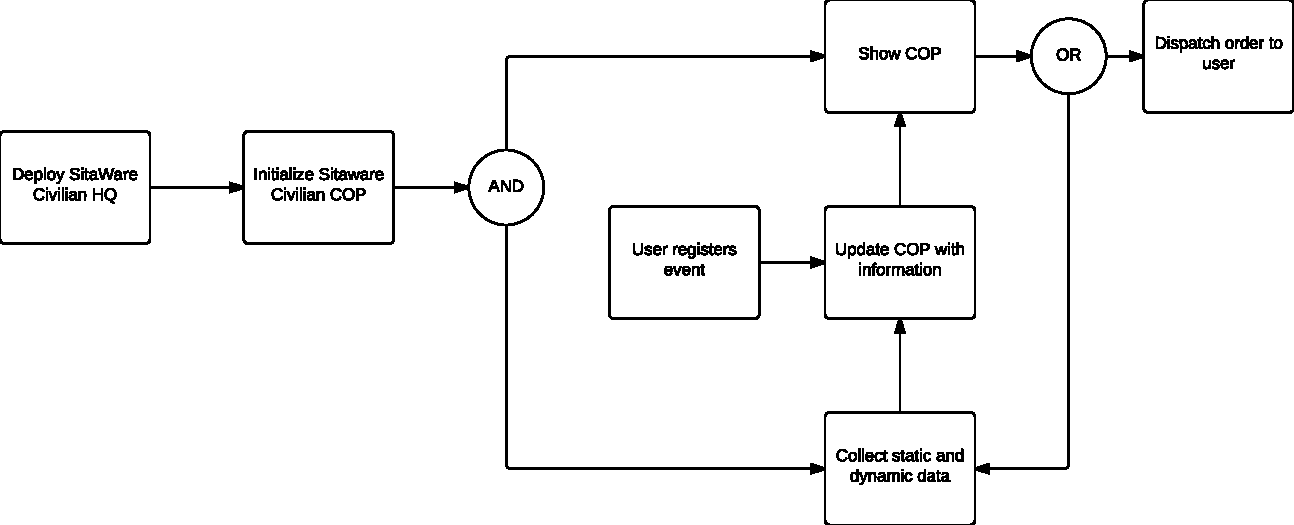
\includegraphics[width=0.95\textwidth]
{billeder/functional_flow_block_diagram.pdf}
\caption{Functional flow block diagram.}
\label{fig:functional_flow_block_diagram}
\end{figure}
\section{Support and Warranty}

In contrast to many software acquisitions, which are typically delivered "as is" and without warranty of any kind, the customer of SitaWare Civilian specifically requests that software shall be covered by warranty. Warranty period shall be at least 10 years. The customer requires the paragraphs in figure \ref{fig:warranty} to be part of the warranty.

\begin{figure}[H]
\centering
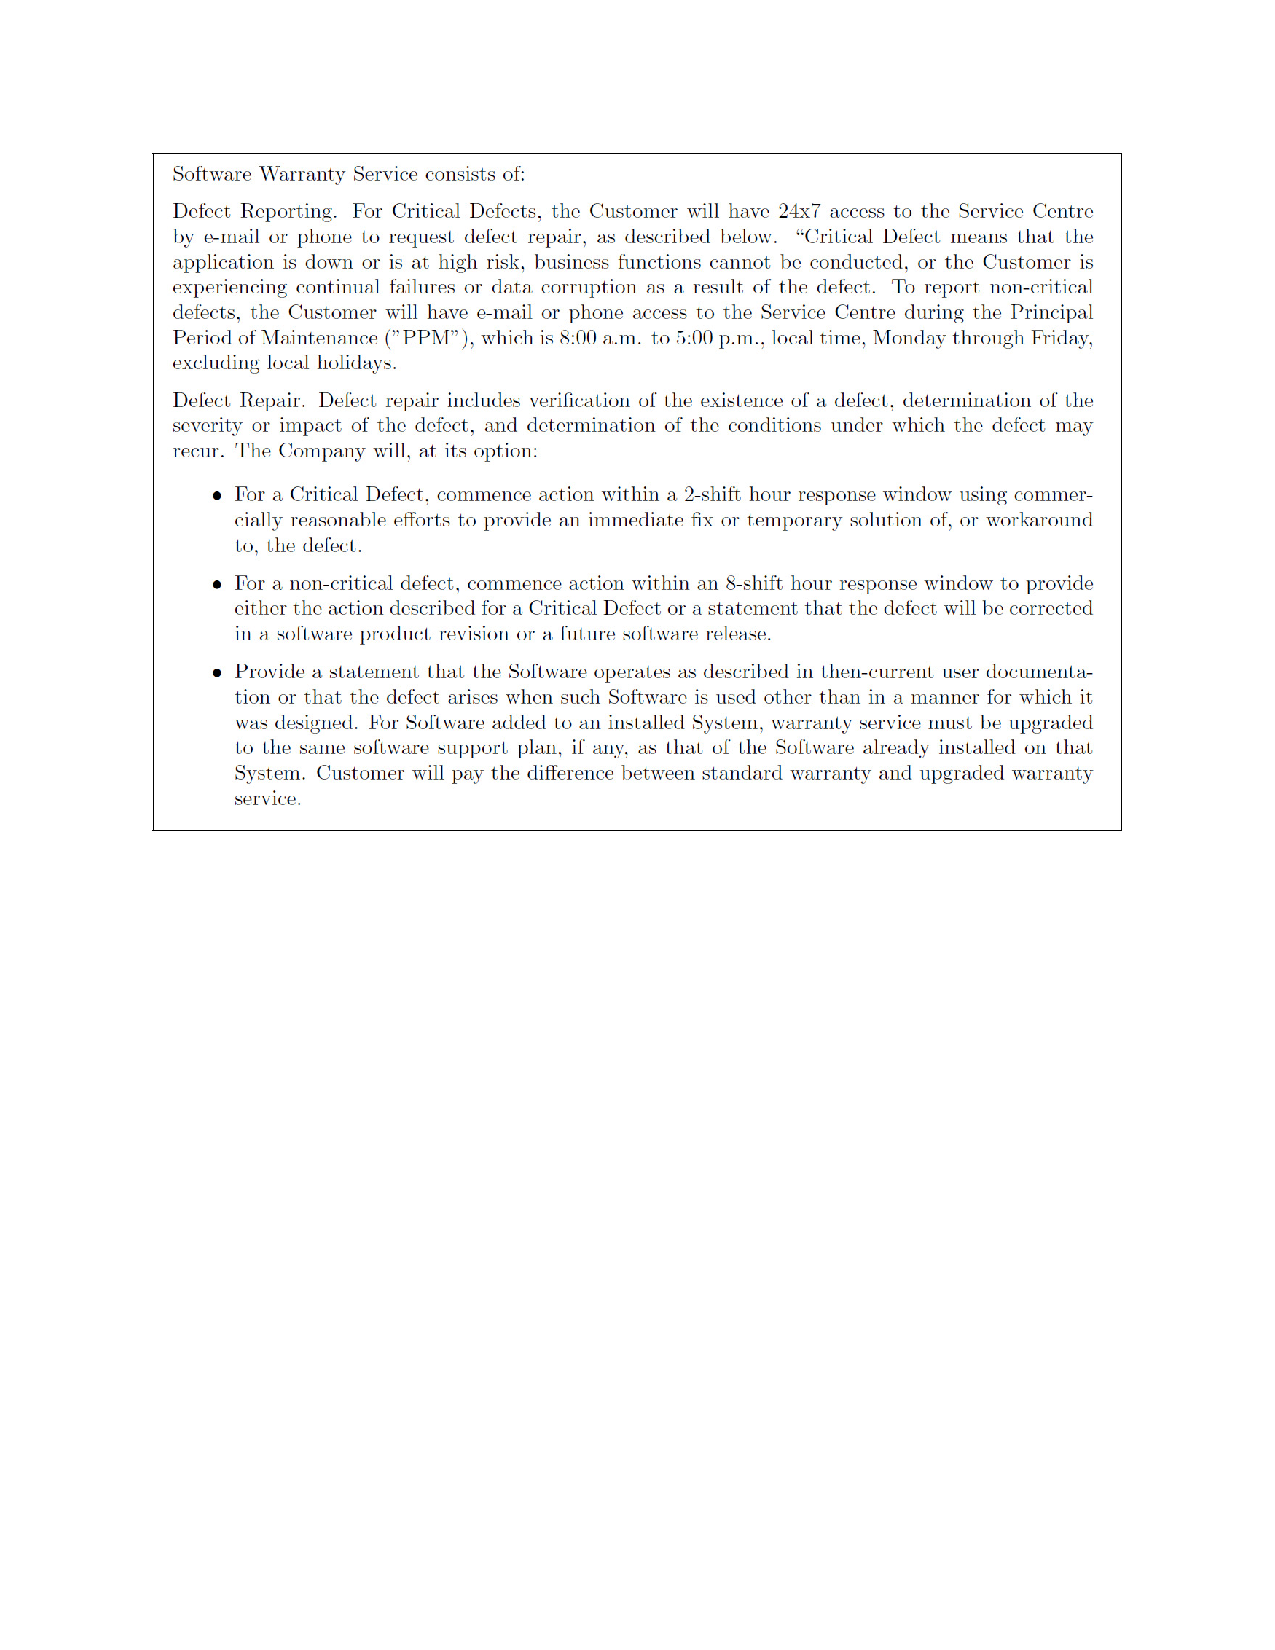
\includegraphics[trim = 25mm 135mm 20mm 25mm, width=0.95\textwidth]
{billeder/warranty.pdf}
\caption{Software Warranty Service.}
\label{fig:warranty}
\end{figure}

%%%% Fixme-listen %%%%
%\newpage										% Ny side til Fixme-listen
%\listoffixmes									% Fixme-listen - fjernes til sidst i projektet med "%"



\end{document}									% Slutter dokumentet - obligatorisk